
% Can also go beyond and define dynamical quantum $SU(n,1)$, starting from one-parameter space of complex projective spaces. Works for all hermitian symmetric spaces


%The relations for the adjoint further imply that \begin{eqnarray*}u_{kl}^{+-} &=&\frac{E(l,l-1)}{E(k,k+1)}(u_{k+1,l-1}^{-+})^*,\\  u_{kl}^{++}&=& \frac{E(l,l+1)}{E(k,k+1)}(u_{k+1,l+1}^{--})^* .\end{eqnarray*}


%\begin{eqnarray*} u_{++} &=& \frac{w_+(\rho)^{1/2}}{w_+(\lambda)^{1/2}}u_{--}^*,\\u_{+-}&=& (-1)^{s_q}  \frac{w_-^{1/2}(\rho)}{w_+^{1/2}(\lambda)}u_{-+}^*.  \\ 
%\end{eqnarray*}

%Let us write \[F(k) = |q|^{-1}w_+(k) =  |q|^{-1}\frac{|q|^{x+k+1}+|q|^{-x-k-1}}{|q|^{x+k}+|q|^{-x-k}},\] and further put\[\alpha = \frac{F^{1/2}(\rho-1)}{F^{1/2}(\lambda-1)}u_{--},\qquad \beta = \frac{1}{F^{1/2}(\lambda-1)}u_{-+}.\] Then the unitarity of $(u_{\epsilon,\nu})_{\epsilon,\nu}$ together with \eqref{EqAdju} and \eqref{EqGradu} are equivalent to the commutation relations \begin{equation}\label{EqqCom} \alpha \beta = qF(\rho-1)\beta\alpha \qquad \alpha\beta^* = qF(\lambda)\beta^*\alpha\end{equation} \begin{equation}\label{EqDet} \alpha\alpha^* +F(\lambda)\beta^*\beta = 1,\qquad \alpha^*\alpha+q^{-2}F(\rho-1)^{-1}\beta^*\beta = 1,\end{equation}\begin{equation*} F(\rho-1)^{-1}\alpha\alpha^* +\beta\beta^* = F(\lambda-1)^{-1},\qquad  F(\lambda)\alpha^*\alpha +q^{-2}\beta\beta^* = F(\rho),\end{equation*} \begin{equation}\label{EqGrad} f(\lambda)g(\rho)\alpha =
%\alpha f(\lambda+1)g(\rho+1),\qquad f(\lambda)g(\rho)\beta = \beta f(\lambda+1)g(\rho-1).\end{equation}%layout might be nicer

%These are precisely the commutation relations for the dynamical quantum $SU(2)$-group as in \cite[Definition 2.6]{KoR1}, except that the precise value of $F$ has been changed by a shift in the parameter domain by a complex constant. Clearly, by Theorem \ref{TheoGenRel} the (total) coproduct on $A_x$ also agrees with the one on the dynamical quantum $SU(2)$-group, namely \begin{eqnarray*} \Delta(\alpha) &=& \Delta(1) (\alpha\otimes \alpha - q^{-1}\beta\otimes \beta^*),\\ \Delta(\beta) &=& \Delta(1)(\beta\otimes \alpha^* +\alpha\otimes \beta)\end{eqnarray*} where $\Delta(1) = \sum_{k\in \Z} \rho_k\otimes \lambda_k$.

%Let us write $B_x = B_x(\Gamma)$ for the $*$-algebra generated by a copy of the $*$-algebra $c_b(\Z\times \Z)$ of bounded functions on $\Z\times \Z$ as well as elements $\alpha,\beta$ satisfying the relations \eqref{EqqCom}, \eqref{EqDet} and \eqref{EqGrad}.

% Lemma doesn't work because $\alpha$,$\beta$ not bounded.
%\begin{Lem} There is a one-to-one correspondence between non-degenerate $*$-representations of $A_x$ on Hilbert spaces and unital $^*$-representations of $B_x$ on Hilbert spaces for which the restriction to $c_b(\Z\times \Z)$ is strictly continuous.
%\end{Lem}


% Give motivation for result coamenability: continuous spectrum can only be in [-2,2], and easy to see universal one has bigger cont. spectrum
\section{The C$^*$-algebras of the dynamical quantum $SU(2)$}\label{SecUni}

\subsection{Definition}

We assume in the following that $0<q<1$ and $\sigma \in \{-1,+1\}$. We also choose $x>0$.
%We also choose $x\in \lbrack \sqrt{q},1\rbrack$.

We recall from \cite{DCT1} the definition of the dynamical $SU(2)$ partial compact quantum group $SU_q(2)_{\dyn,x}$, whose associated partial Hopf $^*$-algebra we denote by $(A_x,\Delta)$. Denote $\ctau(y) = y+y^{-1}$ and $w_{\pm}(y) = \frac{\ctau(q^{\pm 1}y)}{\ctau(y)}$. Denote $\sigma_+ = 1$ and $\sigma_- = -\sigma$. Let $\Lambda_x = xq^{\Z}$, and let $B$ be the $^*$-algebra of finite support functions on $\Lambda_x\times \Lambda_x$, whose Dirac functions we write as $\delta_{(y,z)}=\UnitC{y}{z}$. Then $A_x$ is the $^*$-algebra generated by a copy of $B$ and elements \[(u_{\epsilon,\nu})_{y,z}\] for $\epsilon,\nu\in \{-1,1\}=\{-,+\}$ and $y,z\in \Lambda_x$ with defining relations \begin{eqnarray*} \sum_{\mu\in \{\pm\}} (u_{\mu,\epsilon})_{q^{-\mu}w,y}^* (u_{\mu,\nu})_{q^{-\mu}w,z}&=& \delta_{y,z} \delta_{\epsilon,\nu} \UnitC{w}{q^{\epsilon}y},\\ \sum_{\mu\in \{\pm\}} (u_{\epsilon,\mu})_{y,w} (u_{\nu,\mu})_{z,w}^* &=& \delta_{\epsilon,\nu}\delta_{y,z} \UnitC{y}{w} \\ (u_{\epsilon,\nu})_{y,z}^* &=& \frac{\sigma_{\nu}w_{\nu}(z)^{1/2}}{\sigma_{\epsilon}w_{\epsilon}(y)^{1/2}} (u_{-\epsilon,-\nu})_{q^{\epsilon}y,q^{\nu}z}.\end{eqnarray*} The element $(u_{\epsilon,\nu})_{y,z}$ lives inside the component $\Gr{(A_x)}{y}{q^{\epsilon}y}{z}{q^{\nu}z}$.

Consider $M(A_x)$, the multiplier algebra of $A_x$. For a function $f$ on $\Lambda_x\times \Lambda_x$, write $f(\lambda,\rho) = \sum_{y,z} f(y,z)\UnitC{y}{z} \in M(A_x)$. Similarly, for a function $f$ on $\Lambda_x$ we write $f(\lambda) = \sum_{y,z} f(y)\UnitC{y}{z}$ and $f(\rho) = \sum_{y,z}f(z)\UnitC{y}{z}$. We then write for example $f(q\lambda,\rho)$ for the element corresponding to the function $(y,z)\mapsto f(qy,z)$.

We can further form in $M(A_x)$ the elements $u_{\epsilon,\nu} = \sum_{y,z} (u_{\epsilon,\nu})_{y,z}$. Then $u=(u_{\epsilon,\nu})$ is a unitary 2$\times$2 matrix. Moreover, \begin{equation}\label{EqAdju}u_{\epsilon,\nu}^* = u_{-\epsilon,-\nu}\frac{ \sigma_{\nu}w_{\nu}^{1/2}(\rho)}{\sigma_{\epsilon}w_{\epsilon}^{1/2}(\lambda)}.\end{equation} We then have the following commutation relations between functions on $\Lambda_x\times \Lambda_x$ and the entries of $u$: \begin{equation}\label{EqGradu} f(\lambda,\rho)u_{\epsilon,\nu} = u_{\epsilon,\nu}f(q^{-\epsilon}\lambda,q^{-\nu}\rho).\end{equation}

We will write $u_{--}=\alpha, u_{-+}= \beta, u_{+-}=\gamma,u_{++}=\delta$. We then have the following relations.

\begin{equation}\label{EqId1}\left\{\begin{array}{lllllll} \alpha\alpha^* + \beta\beta^*, &=& 1 &&  \gamma\gamma^* + \delta\delta^* &=& 1,\\ \alpha^*\alpha+ \gamma^*\gamma &=&1,&&\beta^*\beta+ \delta^*\delta &=& 1,\\ \\ \alpha \gamma^* = -\beta \delta^*, &&&& \alpha^*\beta = -\gamma^*\delta, \end{array}\right.\end{equation}

\begin{equation}\label{EqId2} \delta^* = \alpha \frac{w_+^{1/2}(\rho)}{w_+^{1/2}(\lambda)}, \quad \gamma^*=  -\sigma \beta\frac{w_{-}^{1/2}(\rho)}{w_+^{1/2}(\lambda)},\quad  \beta^* = -\sigma \frac{w_+^{1/2}(\lambda)}{w_{-}^{1/2}(\rho)}\gamma, \quad  \alpha^* =  \frac{w_+^{1/2}(\lambda)}{w_+^{1/2}(\rho)}\delta.\end{equation}

The total coproduct $\Delta$ on $A_x$ is then completely determined by the formula \[\Delta(u_{\epsilon,\nu}) = \Delta(1)\left(\sum_{\mu} u_{\epsilon,\mu}\otimes u_{\mu,\nu}\right).\]

%As before, the counit $\epsilon$ gives a $^*$-representation $\weps:A_x \rightarrow B(l^2(\Lambda_x))$ which can again be uniquely characterised, using its extension to $M(A_x)$, by 

%\begin{align*} \weps(\alpha) \delta_y = \delta_{qy},&& \weps(\beta) = 0,&&\weps(f(\lambda,\rho))\delta_y = f(y,y)\delta_y.\end{align*}

%Finally, the antipode $S$ is determined by $S(u_{\epsilon,\nu}) = u_{\nu,\epsilon}^*$ and $S(f(\lambda,\rho)) = f(\rho,\lambda)$. 

% Next piece only for $\sigma = +$!

For completeness, let us also recall the correspondence with the formalism of Koelink and Rosengren \cite{KoR1}. Let us index the generators as they appear in \cite[Definition 2.6]{KoR1} by KR. Moreover, we shift in all their formulas the parameters $\mu$ and $\lambda$ by $\frac{i\pi}{2\ln(q)}$, and after this shift use on $\mathfrak{h}^* \cong \C$ the ordinary complex conjugation as the abstract conjugation $\lambda \mapsto \bar{\lambda}$, cf. the discussion before \cite[Definition 2.8]{KoR1}. Then with $F(y) = \frac{q^{2(y+1)}+q^{-2}}{q^{2(y+1)}+1}$ denoting the (shifted) function appearing at the beginning of section 2.2 in \cite{KoR1}, we have that the correspondence \begin{align*} &\lambda = q^{\lambda_{KR}+1},&& \rho = q^{\mu_{KR}+1},\\ &\alpha = \frac{F^{1/2}(\lambda_{KR}-1)}{F^{1/2}(\mu_{KR}-1)}\alpha_{KR}&& \beta = F^{1/2}(\lambda_{KR}-1)\beta_{KR},\\ &\gamma = F^{-1/2}(\mu_{KR}-1)\gamma_{KR}&& \delta = \delta_{KR}\end{align*} respects the commutation relations of all the generators. 


\subsection{Representation theory of $A_x$}


We wish to classify the irreducible $^*$-representations of $A_x$. We will need an auxiliary notion.

%The parametrisation will hinge on the classification of what we call irreducible $$-adapted sets, which we will now discuss.

%\subsection{Irreducible $c$-sets}

\begin{Def}\label{DefAdapt} Let $c\in\R$. For $\epsilon \in \{\pm\}$, a real number $y>0$ will be called \emph{$c_{\epsilon}$-adapted} if \begin{equation}\label{EqAd+} c \leq \ctau(q^{-\epsilon}y),\end{equation} and \emph{strictly} $c_{\epsilon}$-adapted if this holds strictly. It is called \emph{$c$-adapted} if it is both $c_+$- and $c_-$-adapted. 

A subset $Z$ of $\R^+_0$ is called a \emph{$c$-set} if the following conditions hold: \begin{itemize} 
\item[$\bullet$] $Z$ is not empty.
\item[$\bullet$] $Z$ consists of $c$-adapted points.
\item[$\bullet$] If $y\in Z$ is strictly $c_{\epsilon}$-adapted, then $q^{-2\epsilon}y$ is in $Z$.
\end{itemize}
%An $(x,c)$-set $Z$ is called \emph{even} (resp.~ \emph{odd}) if $Z\subseteq q^{2\Z}$ (resp.~ $Z\subseteq q^{2\Z+1}$).
A $c$-set is called \emph{irreducible} if it can not be written as the union of two disjoint $c$-sets.
\end{Def}

We will classify irreducible $c$-sets. For $y>0$, we write $T_y = yq^{1+2\Z}$, $T_y^+ = yq^{1+2\N}$ and $T_y^{-} = yq^{-1-2\N}$. 

%We use the convention $\N = \{0,1,2,\ldots\}$ and $\N_0=\{1,2,\ldots\}$.

\begin{Prop}\label{PropClass1D}

% Picture!
\begin{itemize} The following list exhausts all irreducible $c$-sets.
\item[$\bullet$] $c<2: T_y$ for $y>0$
\item[$\bullet$] $c \geq 2$, $c=\ctau(z)$ with $0 < z\leq 1$:
\begin{itemize}
\item[$\bullet$] $T_y$ for $\frac{q}{z}<qy<\frac{z}{q}$.
\item[$\bullet$] $T_{z}^+$ and $T_{1/z}^-$.
\item[$\bullet$] $\{1\}$ if $z=q$.
\end{itemize}
\end{itemize}
\end{Prop} 
\begin{proof} Elementary.
\end{proof} 

Let us now turn to the representation theory of the $^*$-algebra $A_x$.

Let $\pi$ be any (necessarily bounded) non-degenerate $^*$-representation of $A_x$ on a Hilbert space $\Hsp_{\pi}$. Then \[\Hsp_{\pi} = \oplus_{y,z} \Hsp^{y}_{z},\qquad \Hsp^{y}_{z} = \pi(\UnitC{y}{z})\Hsp_{\pi}.\] Write \[H_{\pi} =  \textrm{the (non-closed) linear span of all }\Hsp^{y}_{z}.\] Then $\pi(A_x)H_{\pi} = H_{\pi}$. It follows that one can extend $\pi$ to a map \[\pi: M(A_x) \rightarrow \End_{\adj}(H_{\pi}),\] where $\End_{\adj}(H_{\pi})$ denotes the $^*$-algebra of adjointable operators on the pre-Hilbert space $H_{\pi}$. In particular, the generators $\alpha,\beta,\gamma,\delta$ give rise to (contractive) maps $H_{\pi}\rightarrow H_{\pi}$. 

We have the following easy lemma.

\begin{Lem} There is a one-to-one correspondence between\begin{itemize}\item[$\bullet$] non-degenerate $^*$-representations $(\Hsp_{\pi},\pi)$ of $A_x$ on Hilbert spaces, and 
\item[$\bullet$] $\Lambda_x$-bigraded pre-Hilbert spaces $H_{\pi}$ with norm-complete components and equipped with adjointable maps $\alpha,\beta:H_{\pi}\rightarrow H_{\pi}$ satisfying the commutation relations as in \eqref{EqId1} and \eqref{EqId2} and with $f(\lambda,\rho)\xi = f(y,z)\xi$ for $f$ a function on $\Lambda_x\times \Lambda_x$ and $\xi\in H^y_z$.
\end{itemize}
\end{Lem}

\begin{Def} The \emph{Casimir} of $A_x$ is defined to be the following element $\Omega\in M(A_x)$, \[\Omega = \ctau(q\lambda/\rho) - \ctau(\lambda)\ctau(\rho/q)\beta^*\beta.\]  
\end{Def}

\begin{Lem} The element $\Omega$ is a self-adjoint central element in $M(A_x)$.
\end{Lem}
\begin{proof}
This follows from a straightforward calculation. Alternatively, one checks that $\Omega$ is precisely the element $\Xi$ appearing in \cite[Lemma 3.3]{KoR1} under the correspondence mentioned above. 
%By self-adjointness, it suffices to check that $\Omega$ commutes with $\delta^*$ and $\beta^*$. The first commutation follows from the skew commutativity relations and the relation $\ctau(q\lambda)\ctau(\rho)\gamma\gamma^* =\ctau(\lambda)\ctau(\rho/q)\beta^*\beta$. The second commutation follows by using the identity \[\beta\beta^* =  \frac{w_+(\rho/q)-w_+(\lambda/q)}{w_+(\rho/q)} + \frac{w_+(\lambda/q)}{w_+(\rho/q)}\beta^*\beta\] and some elementary computations with the $\tau$-function.
\end{proof}

\begin{Cor}\label{CorCas} If $\pi$ is an irreducible $^*$-representation of $A_x$, there exists $c\in \R$ such that $\pi(\Omega)\xi = c\xi$ for all $\xi \in H_{\pi}$. 
\end{Cor} 
\begin{proof} As $\pi(\Omega)$ is bounded when restricted to any $V^y_z$, this follows immediately from a spectral argument. 
\end{proof} 

Also the following lemma follows from a straightforward computation using the defining relations.

\begin{Lem}\label{LemAmp} Inside $M(A_x)$, we have the following identities:
\begin{align*}
&\alpha^*\alpha = \frac{\ctau(q\lambda\rho)+\Omega}{\ctau(\lambda)\ctau(q\rho)} && \alpha\alpha^* = \frac{\ctau(\lambda\rho/q)+\Omega}{\ctau(\lambda/q)\ctau(\rho)}\\ 
&\beta^*\beta = \frac{\ctau(q\lambda/\rho)-\Omega}{\ctau(\lambda)\ctau(\rho/q)}&& \beta\beta^* = \frac{\ctau(\lambda/q\rho)-\Omega}{\ctau(\lambda/q)\ctau(\rho)}.
\end{align*}
\end{Lem}


\begin{Cor}\label{CorOneDim} If $\pi$ is an irreducible $^*$-representation of $A_x$ on a Hilbert space $\Hsp_{\pi}$, then $\Hsp^y_z$ is at most one-dimensional for each $y,z\in \Lambda_x$. Moreover, either all $\Hsp^y_z$ with $y/z\in q^{2\Z+1}$ are zero, or all $\Hsp^y_z$ with $y/z\in q^{2\Z}$ are zero. 
\end{Cor} 
\begin{proof} 
Using Corollary \ref{CorCas}, these assertions follow immediately from the defining relations and Lemma \ref{LemAmp}.
\end{proof}

%\begin{Def} Let $(\Hsp_{\pi},\pi)$ be an irreducible $^*$-representation of $A_x$. We call $\pi$ even (resp. odd) if all $\Hsp^y_z$ with $y/z \in q^{2\Z+1}$ (resp.~ $q^{2\Z}$) are zero.
%\end{Def} 

%We can hence identity $\Hsp$ as a quotient of $l^2(\Z\times \Z)$. Write the images of the standard basis vectors $e_{m,n}$ of $l^2(\Z\times \Z)$ as $f_{m,n}$. Let us write $F = \{(m,n)\mid f_{m,n}\neq 0\}$.

With the above preliminaries, we can now classify the irreducible $^*$-representations of $A_x$. We first extend the terminology of Definition \ref{DefAdapt}.
% Different order of introducing?


\begin{Def} Fix $c\in \R$. For $\epsilon,\nu\in \{-,+\}$, a couple $(y,z)$ of strictly positive reals is called \emph{$c_{\epsilon,\nu}$-adapted} if the following inequality holds: \begin{equation}\label{EqAd} \ctau(q^{-\epsilon}yz^{\epsilon\nu})+\epsilon\nu c\geq 0.\end{equation} A couple $(y,z)$ is called \emph{strictly} $c_{\epsilon,\nu}$-adapted if this is a strict equality. We call $(y,z)$ \emph{$c$-adapted} if it is $c_{\epsilon,\nu}$-adapted for all $\epsilon,\nu\in \{+,-\}$. 
\end{Def} 

\begin{Def} Fix $c\in \R$. We call a subset $T\subseteq \R_{>0}^2$ a \emph{$c$-set} if the following conditions are satisfied: 
\begin{itemize} 
\item[$\bullet$] $T$ is not empty.
\item[$\bullet$] $T$ consists of $c$-adapted points.
\item[$\bullet$] If $(y,z)\in T$ is strictly $c_{\epsilon,\nu}$-adapted, then $(q^{-\epsilon}y,q^{-\nu}z)$ is in $T$.
\end{itemize}

We say that $T$ is \emph{irreducible} if it is not the disjoint union of two $c$-sets.

%Writing $\Z^2_{\even} = \{(k,l)\mid k-l \textrm{ even}\}$ and $\Z^2_{\odd} = \Z^2\setminus \Z^2_{\even}$, we call an $(x,c)$-set even or odd according to whether it lies in $\Z^2_{\even}$ or $\Z^2_{\odd}$.
\end{Def}

\begin{Def} Fix $x>0$. For $\pi$ an irreducible representation of $A_x$, a couple $(y,z)\in \Lambda_x\times \Lambda_x$ is called $\pi$-compatible if $\Hsp^y_z\neq 0$. 

For $c\in \R$, a subset $T\subseteq \Lambda_x\times \Lambda_x$ is called \emph{$(x,c)$-compatible} if there exists an irreducible representation $\pi$ of $A_x$ with $\pi(\Omega) = c$ and $T=\{(y,z)\in \Lambda_x\times \Lambda_x\mid \Hsp^{y}_{z}\neq \{0\}\}$. In this case, we say that $\pi$ is \emph{$T$-adapted}.
\end{Def}

\begin{Prop}\label{PropClassRep} A set $T\subseteq \Lambda_x\times \Lambda_x$ is an irreducible $c$-set if and only if it is an $(x,c)$-compatible set. Moreover, for any $(x,c)$-compatible set $T$ there is exactly one irreducible $^*$-representation $\pi$ of $A_x$, up to unitary equivalence, which is $T$-compatible.
\end{Prop}

\begin{proof} Assume first that $T$ is $(x,c)$-compatible, and let $\pi$ be a $T$-compatible irreducible $^*$-representation of $A_x$. If $(y,z)\in T$, then it follows from Lemma \ref{LemAmp} that $(y,z)$ is $c$-adapted. Moreover, if $(y,z)\in T$ is strictly $c_{\epsilon,\nu}$-adapted, then we have that $\|u_{\epsilon,\nu}\xi\|\neq 0$ for a non-zero $\xi\in \Hsp^y_z$, hence also $\Hsp^{q^{-\epsilon}y}_{q^{-\nu}z}\neq \{0\}$. It follows that $T$ is a $c$-set. Now if $T=T_1\cup T_2$ a disjoint union of $c$-sets, it would follow that $\pi$ restricts to the direct sum of all $\Hsp^y_z$ with $(y,z)\in T_1$, contradicting irreducibility. It follows that $T$ is an irreducible $c$-set.

Conversely, let $T$ be an irreducible $c$-set inside $\Lambda_x\times \Lambda_x$. Put $\Hsp_{\pi} = l^2(T)$ with \begin{eqnarray*} \pi(\alpha)  \delta_{y,z} &=&  \left(\frac{\ctau(qyz)+c}{\ctau(y)\ctau(qz)}\right)^{1/2}\delta_{qy,qz},\\ \pi(\beta) \delta_{y,z} &=& \sigma_y\left(\frac{\ctau(qy/z)-c}{\ctau(y)\ctau(z/q)}\right)^{1/2} \delta_{qy,z/q},\end{eqnarray*} where the right hand side is considered as the zero vector when the scalar factor on the right is zero, and where $\sigma_y = \sigma$ if $y\in xq^{2\Z+1}$ and $1$ otherwise. Note that the roots on the right hand side are well-defined precisely because $T$ is a $c$-set. 

By direct computation, using the defining commutation relation, we see that $\pi$ defines a $^*$-representation of $A_x$ with $\pi(\Omega) =c$. Moreover, $\pi$ is irreducible since otherwise, by Corollary \ref{CorOneDim}, $T$ would split as a disjoint union of $(x,c)$-compatible sets. Hence $T$ is an $(x,c)$-compatible set.

Now the formulas for $\pi(\alpha)$ and $\pi(\beta)$ are uniquely determined up to a unimodular gauge factor. As any non-zero $\Hsp^{y}_z$ is cyclic for $\pi$, it follows that these gauge factors are determined by their value at one component. As the $\alpha$ and $\beta$ define different shifts in the grading, we then easily conclude that $\pi$ is in fact the unique $T$-compatible $^*$-representation, up to unitary equivalence.
\end{proof}

What remains is to classify irreducible $c$-sets for each $c\in \R$. 

\begin{Lem}\label{LemClass2D} A set $T\subseteq \R_{>0}^2$ is an irreducible $c$-set if and only if there exists an irreducible $-c$-set $Z_+\subseteq \R_{>0}$ and an irreducible $c$-set $Z_-\subseteq \R_{>0}$ such that $(y,z)\in T$ if and only if $yz\in Z_+$ and $y/z\in Z_-$.
\end{Lem} 

\begin{proof} It is immediate that $(y,z)\in \R_{>0}^2$ is (strictly) $c_{\epsilon,\nu}$-adapted if and only if $yz^{\epsilon\nu}$ is (strictly) $(-\epsilon\nu c)_{\epsilon}$-adapted. The conclusion of the lemma then follows immediately.
\end{proof}

Let now $\mathcal{A}_x$ be the universal C$^*$-envelope of $A_x$. As the $\Omega\UnitC{y}{z}$ define orthogonal bounded elements in $A_x\subseteq \mathcal{A}_x$, we can make sense of $\Omega$ as an element affiliated to $\mathcal{A}_x$, i.e. $\Omega\,\eta\,\mathcal{A}_x$ \cite{Wor2}. 

\begin{Cor} Let $k_0\in \Z$ be the unique integer such that $q^{k_0+1}<x^2\leq q^{k_0}$, and write $z_{0} = \min \{q^{-k_0}x^2,q^{k_0+1}x^{-2}\}$. Then the spectrum of $\Omega \in \mathcal{A}_x$ equals the set \[\Spec(\Omega) = \lbrack -\tau(z_0),q+q^{-1}\rbrack \cup q^{\Z}\cup (-x^2q^{\Z}) \cup (-x^{-2}q^{\Z}).\]
\end{Cor}
\begin{proof} We have that $c \in \Spec(\Omega)$ iff there exists an irreducible $c$-set $\subseteq \Lambda_x\times \Lambda_x$. If $c\geq 0$, this is equivalent with the existence of an irreducible $c$-set $Z_- \subseteq q^{\Z}$, while if $c\leq 0$ this is equivalent with the existence of an irreducible $-c$-set $Z_+ \subseteq x^2q^{\Z}$. But for $c\geq0$ and $y>0$, there exists an irreducible $c$-set $Z\subseteq yq^{\Z}$ iff either $c<2$ or $c=\tau(z)$ for some $0<z\leq 1$ with either ($\frac{q}{z}\leq qy' \leq \frac{z}{q}$ for some $y'\in yq^{\Z}$) or ($z$ or $1/z \in yq^{\Z}$). It is elementary to verify that this leads to the spectrum as stated in the corollary.
\end{proof}


%Combining Proposition \ref{PropClassRep} with Proposition \ref{PropClass1D} and Lemma \ref{LemClass2D}, we thus obtain a concrete description of the spectrum of $A_x$. The following pictures illustrate the form of the spectrum of $A_x$ for the case $q>0$.

%\begin{figure}[h]
%  \centering
%\input{specx0-even.epic}
%  \caption{Case $x=0$, even}
%\label{figy}
%\end{figure}

% Probably in figure below the middle dot at $-t_0$ should be unfilled!
%\begin{figure}[h]
 % \centering
%\input{specx0-odd.epic}
 %% \caption{Case $x=0$, odd}
%\label{figy}
%\end{figure}


%\begin{figure}[h]
 % \centering
%\input{specx12-even.epic}
 % \caption{Case $x=\frac{1}{2}$, even}
%\label{figy}
%\end{figure}


%\begin{figure}[h]
 % \centering
 % \input{specx12-odd.epic}
  %  \caption{Case $x=\frac{1}{2}$, odd}
%\label{figy}
%\end{figure}

% Should be latexed?
%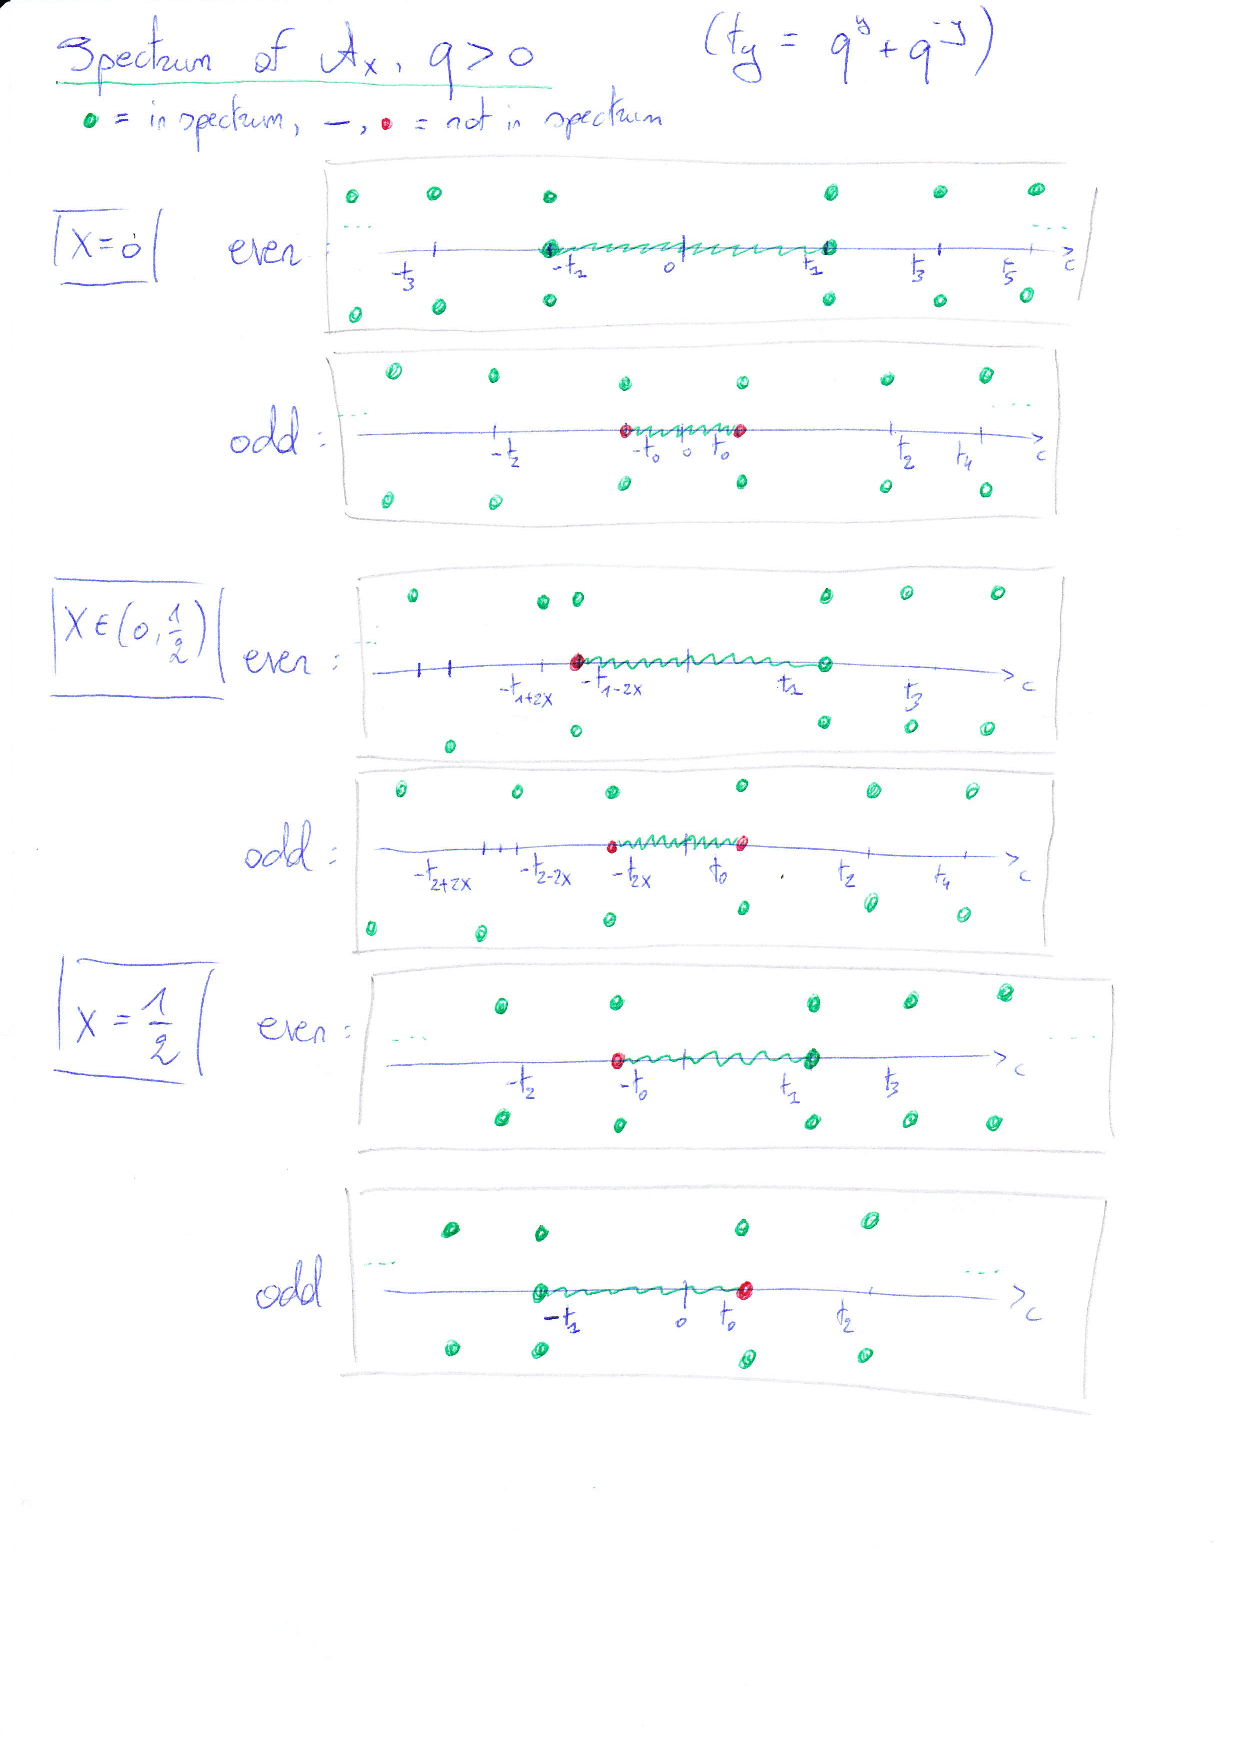
\includepdf[pages={1}]{ScanSpec.pdf}


% Make remark on regular representation cf. Koelink-Rosengren

% Include a concrete descripition of the universal envelope of $A_x$ from this?


%More generally, 

%As a concrete instance of the example of monoidal equivalence, let $\tilde{A}$ be the generalized compact Hopf face algebra obtained from the set $\tilde{I} =I_1\sqcup I_2$ with $I_1= \Z$ and $I_2= \{\bullet\}$ with the $B_{kl} =\emptyset$ and $E(k,l)$ for $k,l\neq \bullet$ as in section ..., with $B_{k,\bullet} = B_{\bullet,k}= \emptyset$, and $B_{\bullet,\bullet} = \{\pm\}$ with $E_{\bullet,\bullet} = \begin{pmatrix} 0 & |q|^{1/2} \\ -\sgn(q)|q|^{-1/2}&0\end{pmatrix}$ (with the basis ordered as $-,+$). Then this will be obtained from the direct sum of the functor from ... and the ordinary forgetful functor from $\Rep(SU_q(2))$ into $\Hilb$. It follows that the components $\tilde{A}(ij)$ can be described by the generators and relations as in ..., but with $F(\lambda)$ and $F(\rho)$ set equal to 1 whenever the corresponding index is $\bullet$.




% Study spectrum fundamental character
% Study dual quantum groupoid
% Make connection with dynamical cocycle
% In case of qgroupoid constructed from identity functor for Rep(SU_q(2)): rep theory of associated Galois object should just be: a single representation (Galois object is type I factor, cutdown of $B(\mathscr{L}^2(SU_q(2)))$). Yes: in general, Galois object is Morita equivalent with algebra of original ergodic action, should also be stressed for Podles spheres

\subsection{The reduced C$^*$-algebra of the dynamical quantum $SU(2)$ group}

% Notation $\weps$ should be recalled?
In \cite{KoR1}, the corepresentation theory of the dynamical quantum $SU(2)$ group is investigated. Transporting their definition to our setting, an $n$-dimensional corepresentation consists of $n^2$ elements $t_{kl} \in M(A_x)$, together with an assigment $k \mapsto q_k \in q^{\Z}$ such that \begin{align*} \Delta(t_{km}) = \Delta(1)\left(\sum_{l=1}^n t_{kl}\otimes t_{lm}\right)&& \weps(t_{kl})\delta_y = \delta_{kl} \delta_{q_ky},&& f(\lambda,\rho)t_{kl} = t_{kl}f(q_k\lambda,q_l\rho).\end{align*} Moreover, the corepresentation is called \emph{unitary} if $S(t_{ij})^* =t_{ji}$. To relate this to the theory of corepresentations defined in \cite{DCT1}, put \[\left(\Gr{t}{y}{z}{v}{w}\right)_{kl} = \delta_{y}(\lambda)\delta_v(\rho) t_{kl} \delta_{z}(\lambda)\delta_{w}(\rho).\] Then this defines a unitary corepresentation in the sense of $\cite{DCT1}$ on the collection of vector spaces $V_{y,z}$ where $V_{y,z}=\{0\}$ except when there exists $k$ with $y = q_kz$,  in which case $V_{y,z} = \mathbb{C}^n$ (and with the matrix coefficients with respect to the canonical basis). 

According to \cite{KoR1}, there is a unitary $2N+1$-dimensional corepresentation $t^N$ for each half-integer $N$ (dropping the tilde appearing in \cite{KoR1}), and moreover the fusion rules of the $t^N$ are as for $SU(2)$. As the tensor products of corepresentations in the sense of \cite{KoR1} and \cite{DCT1} are compatible, we deduce from the abstract theory of \cite{DCT1} that the $t^N$ also form a maximal family of non-equivalent irreducible unitary corepresentations in the sense of \cite{DCT1}. %Moreover, we can label the bases of our vector spaces by integers or halfintegers in such a way that $f(\lambda,\rho)t_{kl}^N = t_{kl}^Nf(q^{-k}\lambda,q^{-l}\rho)$. 
As a concrete example, we have that the generating matrix $(u_{\epsilon,\nu})$ is a unitary corepresentation.

%From the general theory of \cite{DCT1}, we infer that the $\delta_y(\lambda)\delta_z(\rho)t_{kl}^N$ form an orthogonal (but not necessarily orthonormal) basis of $L^2(SU_q(2)_{\dyn})$. 

It then follows straightforwardly from \cite[Section 7]{KoR1} that, with $\varphi_{y,z}$ denoting the Haar functional on $\Gr{A}{y}{y}{z}{z}$, \[\varphi_{y,z}(p(\Omega)) = \int_{\R} p(x)\rd m_{y,z},\] where $m_{y,z}$ is the normalized orthogonality measure for the (rescaled) Askey-Wilson polynomials \[p_k(x) = p_k(2x;qz/y,qy/z,-qyz,-q/yz;q^2).\] From \cite[Theorem 2.1 and Theorem 2.5]{AsW1}%see also Koelink-Verding
, it follows that $m_{y,z}$ has support on the union of the interval $\lbrack -2,2\rbrack$ with the set \[D_{y,z} = \{\tau(eq^k)\mid e\in \{qz/y,qy/z,-qyz,-q/yz\}, k\geq 0, |eq^k|>1\}.\]

In particular, we deduce the following corollary.

\begin{Cor} The spectrum of $\Omega \,\eta\, \CrG$ equals $\lbrack -2,2\rbrack \cup q^{\Z} \cup (-x^2q^{\Z})\cup (x^{-2}q^{\Z})$.
\end{Cor} 

In particular, as this spectrum is strictly smaller than the spectrum of $\Omega$ in $\CuG$, we obtain the following theorem.

\begin{Theorem} The partial compact quantum group $SU_q(2)_{\dyn,x}$ is not coamenable.
\end{Theorem} 




%%% Local Variables: 
%%% mode: latex
%%% TeX-master: "dyn-suq-main"
%%% End: 
